\chapter{Software Testing}

Testing for SwiftBite covered the frontend and backend builds, registration validation, visible prototype workflows, and the working MySQL integration. A read-only query succeeded, the schema was initialized, and the restaurant API was confirmed to return MySQL-backed records. Full authentication and order-persistence integration tests were not performed.

\section{Test Plan and Objectives}

The verification plan covered:
\begin{itemize}
    \item Compilation of the frontend and backend TypeScript projects.
    \item Direct MySQL connectivity, schema initialization, and the database-backed restaurant API response.
    \item Presence and use of the sign-up confirm-password field.
    \item Client-side handling of empty and mismatched registration values.
    \item Rendering of the customer home, menu, checkout, order-status, chatbot, and portal-switcher screens.
    \item Clear identification of the checkout, order, and portal flows as demonstrations rather than live production integrations.
\end{itemize}

\section{Testing Methodologies}

\subsection{Build and Type Checking}
The frontend production build, frontend TypeScript check, and backend TypeScript build were run to identify compilation and type errors.

\subsection{Manual Browser Verification}
The current frontend was opened in a browser. The sign-up screen was checked with mismatched password values, and the resulting validation message was confirmed. Screenshots in this report were captured from the current frontend. These checks do not substitute for automated end-to-end testing against a configured production API.

\subsection{MySQL and API Verification}
A read-only \texttt{SELECT 1} query succeeded against MySQL. The eight-table schema was initialized with four restaurants and four categories. \texttt{GET /api/restaurants} returned four records with the response source identified as MySQL. Registration, login, and persistent order creation were not exercised in this verification.

\section{Test Cases and Results}

\begin{table}[H]
\centering
\caption{Verification Cases}
\label{tab:test_cases}
\renewcommand{\arraystretch}{1.35}
\begin{tabular}{|l|p{3.4cm}|p{6.5cm}|l|}
\hline
\textbf{ID} & \textbf{Feature} & \textbf{Verification} & \textbf{Result} \\
\hline
TC\_01 & Frontend build & Run \texttt{npm run build} in the frontend project. & PASS \\
\hline
TC\_02 & Frontend types & Run \texttt{npx tsc --noEmit} in the frontend project. & PASS \\
\hline
TC\_03 & Backend types & Run \texttt{npm run build} in the backend project. & PASS \\
\hline
TC\_04 & Password confirmation & Enter two different password values in sign-up and submit; the UI displays a mismatch error and does not send the registration request. & PASS \\
\hline
TC\_05 & Prototype screens & Open the current home, restaurant menu, checkout, tracking, chatbot, and portal-switcher interfaces. & PASS \\
\hline
TC\_06 & MySQL connection and schema & Run a read-only query, initialize the schema, and confirm the restaurant API returns database-backed records. & PASS \\
\hline
TC\_07 & Auth/order integration & Exercise registration, login, and persistent order flows against the backend and MySQL instance. & NOT RUN \\
\hline
\end{tabular}
\end{table}
\newpage
\subsection{Password Confirmation Validation}
\textbf{Objective:} Confirm that the registration form does not proceed when the two password fields differ. \\
\textbf{Result:} The browser displayed both the inline mismatch message and the form error; the registration request was not submitted. Figure \ref{fig:password_validation} shows this validation state.

\begin{figure}[H]
    \centering
    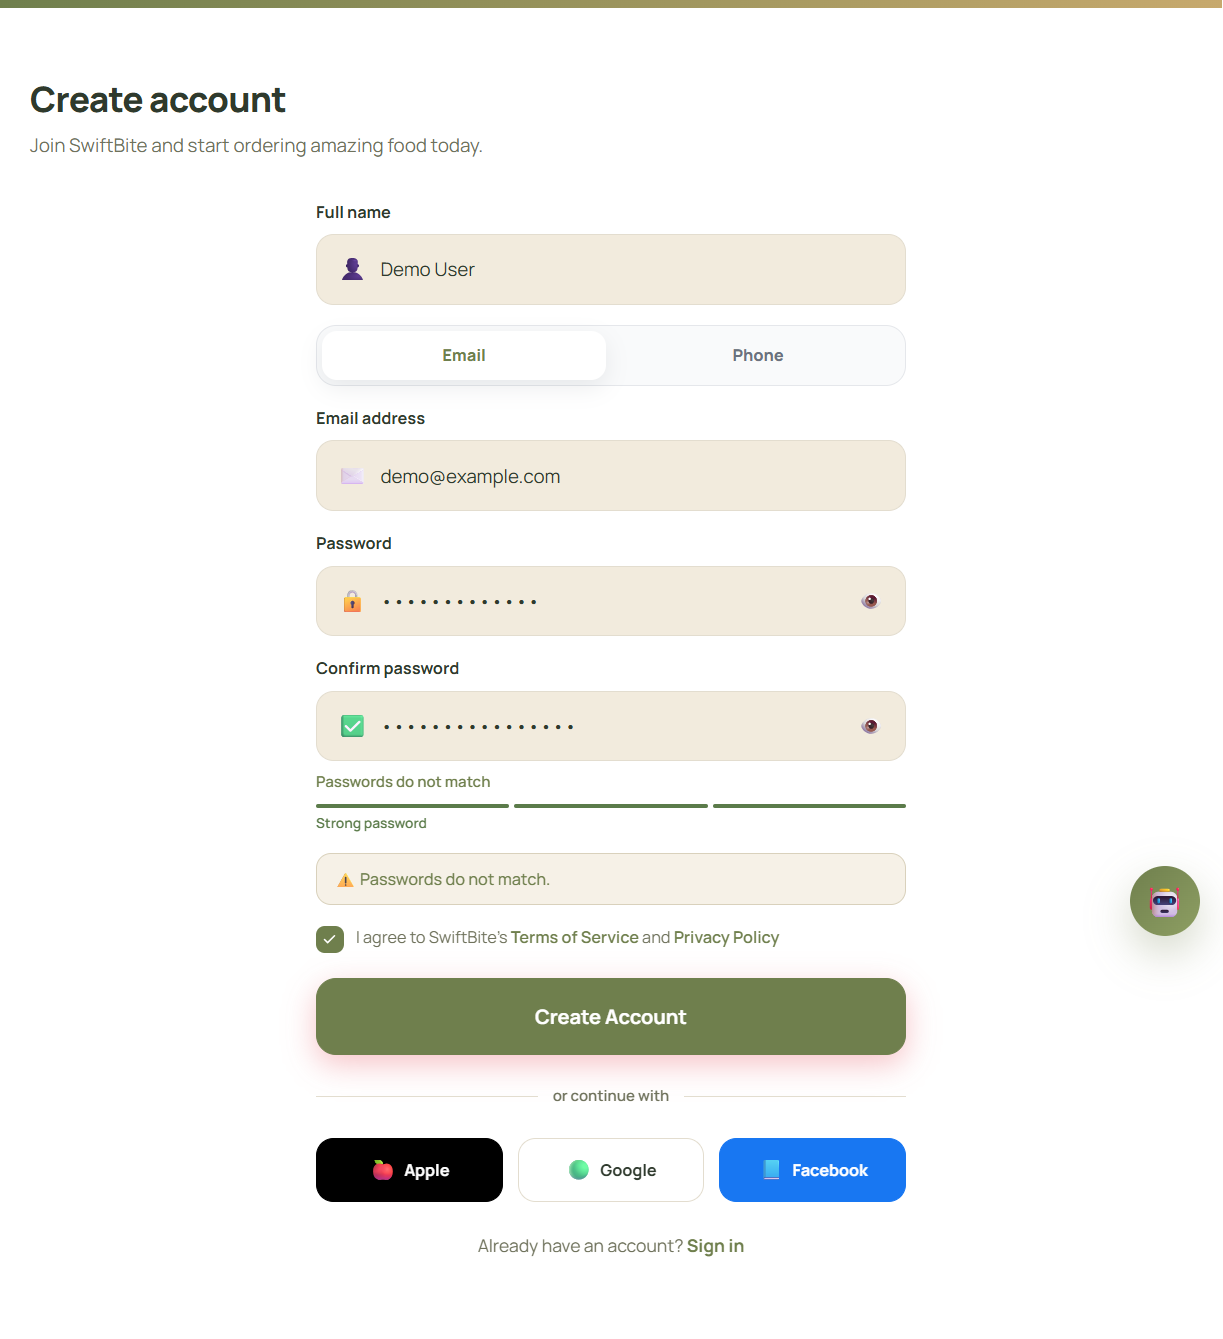
\includegraphics[width=0.72\textwidth,height=0.62\textheight,keepaspectratio]{Chapters/validation_error.png}
    \caption{Sign-up form rejecting mismatched passwords}
    \label{fig:test_validation}
\end{figure}

\subsection{Registration Form}
\textbf{Objective:} Verify the current sign-up fields and required confirmation entry. \\
\textbf{Result:} The current screen presents name, email or phone selection, password, confirm password, and terms acceptance. Successful registration against a live backend was not verified in this browser session.

\begin{figure}[H]
    \centering
    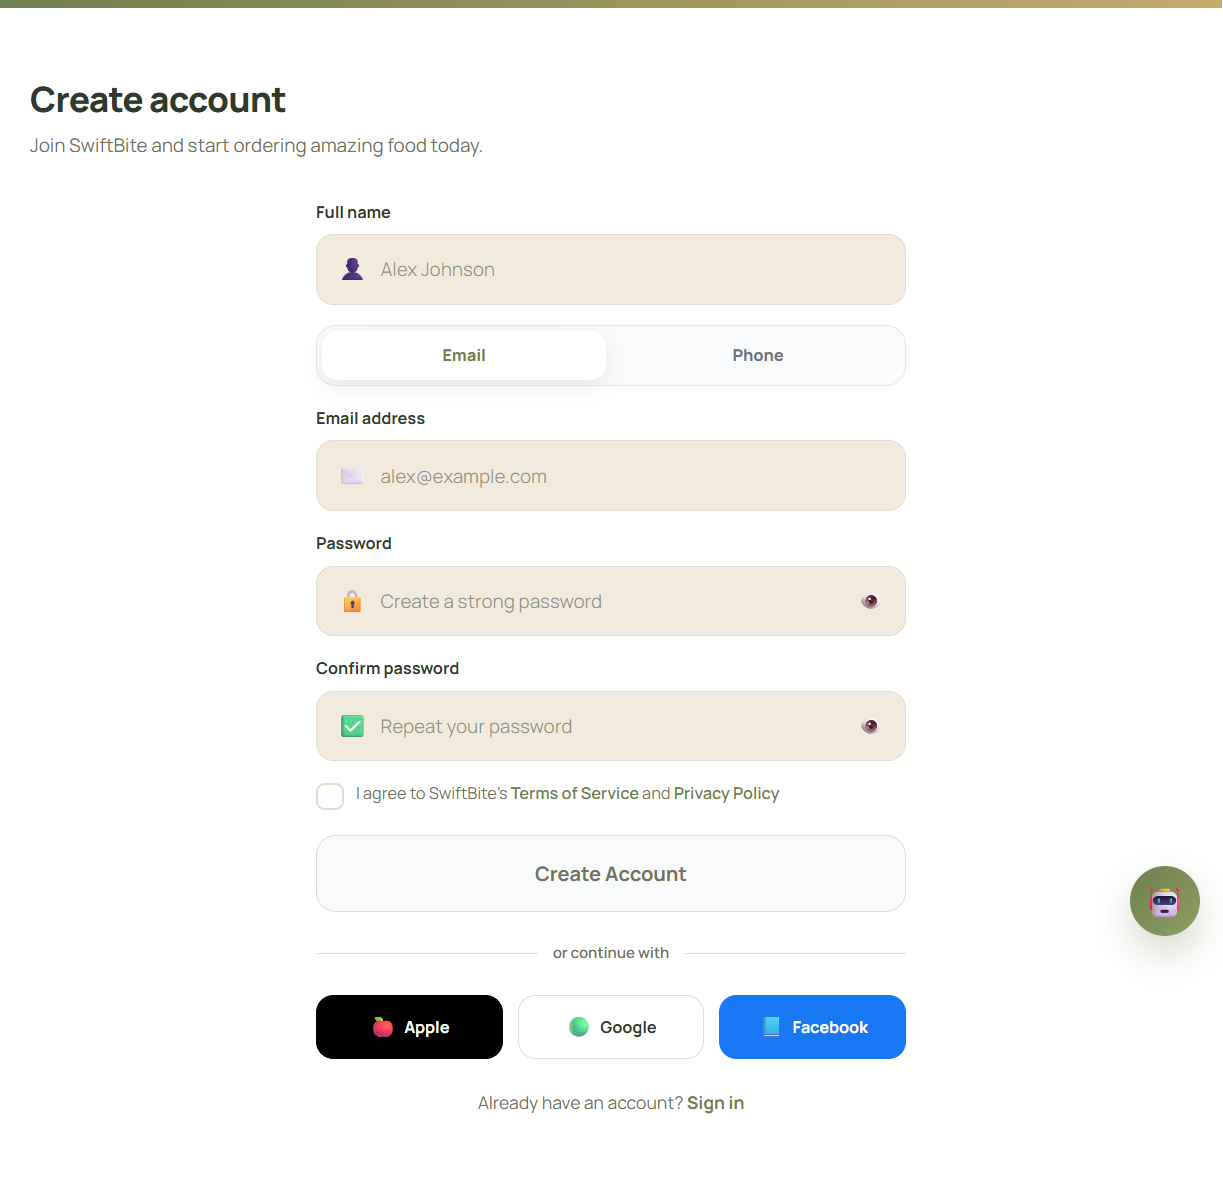
\includegraphics[width=0.72\textwidth,height=0.62\textheight,keepaspectratio]{Chapters/register.png}
    \caption{Current SwiftBite sign-up form}
    \label{fig:test_register}
\end{figure}

\subsection{Scope of Verification}
The customer menu, checkout, order-status, and portal-switcher interfaces render in the browser. The MySQL connection, schema, and restaurant-list API were verified, but the customer catalogue still uses bundled sample data. Checkout does not persist orders or charge a payment method, and the tracking screen does not use GPS. Registration, login, and order-writing routes require separate integration tests.

\section{Testing Conclusion}

The frontend and backend builds and TypeScript checks completed successfully, the sign-up password-mismatch validation was confirmed in the browser, and MySQL connectivity and the restaurant API were verified. These checks do not establish persistent customer ordering, payment processing, GPS tracking, or production authentication behavior.
